\subsubsection{Real-time Communication with SignalR}

The application's real-time updates are handled using SignalR. A dedicated service, \texttt{signalrService.ts}, encapsulates the connection logic. A key implementation detail is securing the SignalR connection through the use of an \texttt{accessTokenFactory}. This function is invoked by the SignalR client whenever an access token is required and retrieves a valid JWT access token from MSAL using the current user context. 

Once the token is retrieved, it is included in the connection request, ensuring that the real-time communication channel is authenticated and authorized. Refer to Figure \ref{fig:msal-signalr} for the \texttt{signalrService.ts} code snippet that demonstrates the \texttt{accessTokenFactory} implementation.


\begin{figure}[H]
    \centering
    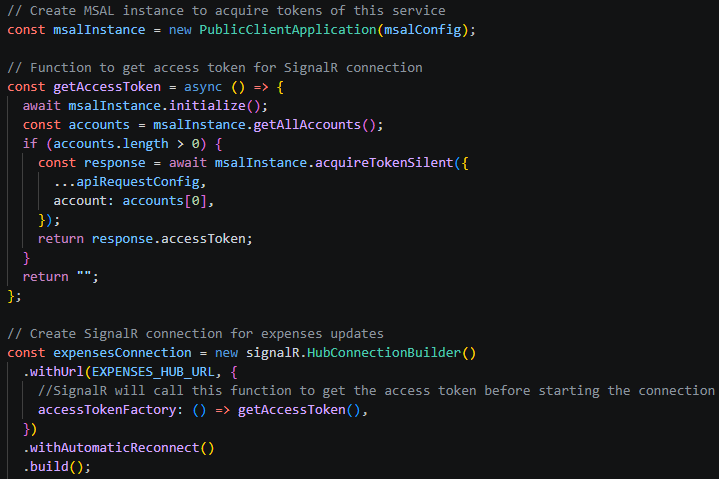
\includegraphics[width=0.7\textwidth]{Images/Implementation/MsalSignalR.png}
    \caption[AccessTokenFactory implementation in signalrService.ts]
    {\texttt{AccessTokenFactory} implementation in \texttt{signalrService.ts}.[Own creation]}
    \label{fig:msal-signalr}
\end{figure}

Once the connection is established, the service subscribes to specific events broadcast by the server hub. The following code (Figure \ref{fig:signalr-events}) shows how the frontend listens for the \texttt{``ExpenseProcessed''} and \texttt{``ExpenseProcessingFailed''} events and triggers a function to update the user interface accordingly.


\begin{figure}[H]
    \centering
    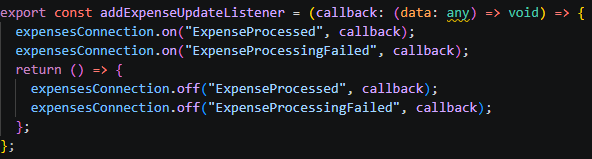
\includegraphics[width=0.7\textwidth]{Images/Implementation/signalREventHubs.png}
    \caption[SignalR event subscription implementation]
    {SignalR event subscription implementation. [Own creation]}
    \label{fig:signalr-events}
\end{figure}